\documentclass[12pt,a4paper,notitlepage,colorinlistoftodos]{article}
%%%%%%%%%%%%%%%%%%%%%%%%%%%%%%%%%%%%%%%%%%%%%%%%%%%%%%%%%%%%%%%%%%%%%
% Template pour rendus Master
%%%%%%%%%%%%%%%%%%%%%%%%%%%%%%%%%%%%%%%%%%%%%%%%%%%%%%%%%%%%%%%%%%%%%%
\usepackage[utf8]{inputenc} %encodage
\usepackage[T1]{fontenc}

\usepackage[square,sort,comma,numbers]{natbib} % bibliography
\setcitestyle{authoryear,open={(},close={)}}
\renewcommand{\bibsection}{}

\usepackage[french]{babel} % langue
% add '\-' to create custom hypernation if a word is difficult to cut or :
\hyphenation{geo-graphique}

%mise en page générale
\usepackage{geometry}
%\geometry{a4paper} % format de feuille
\geometry{top=2.5cm, bottom=2.5cm, left=2.5cm, right=2.5cm} %marges
\usepackage{mathptmx} % Police Times si compilateur pdfLatex
\usepackage{amsmath,amsthm,amssymb}
\usepackage{times}
\setlength{\parindent}{0pt}

\linespread{1} % interligne
\usepackage{fancyhdr} %en tete et pied de page
\usepackage{lastpage}  %marche pas chez julia
\pagestyle{plain} 

\usepackage{lscape} % page en landscape

\usepackage{multicol}
\usepackage{hhline}
\setlength{\columnsep}{1cm}

\usepackage{hyperref,url} % lien cliquables
\hypersetup{
colorlinks = true,
linkcolor = black,
urlcolor = RoyalBlue
}
\usepackage{lipsum} %Lorem ipsum

\usepackage{wrapfig} %position d'images dans le texte
\usepackage{graphicx, subcaption, setspace, booktabs, wrapfig}

\usepackage[table,dvipsnames]{xcolor}

\usepackage{caption}
\DeclareCaptionType{annexe}[Annexe][Liste d'annexes] % rajout pour captions annexes
\DeclareCaptionType{web}[Web][Sites Web] % rajout pour mettre des captions web

\usepackage{todonotes} % notes et commentaires
%\usepackage[disable]{todonotes} % pour supprimer les commentaires lors de la compil

\usepackage[export]{adjustbox}

\usepackage[para,online,flushleft]{threeparttable}


\usepackage{listings}
\usepackage{color}
 
%http://latexcolor.com/ 
\definecolor{codegray}{rgb}{0.5,0.5,0.5}
\definecolor{cerulean}{rgb}{0.0, 0.48, 0.65}
\definecolor{beaublue}{rgb}{0.95, 0.95, 0.95}
\definecolor{amber}{rgb}{1.0, 0.25, 0.0}
\definecolor{indiagreen}{rgb}{0.07, 0.53, 0.03}
\definecolor{number}{rgb}{0.01, 0.01, 0.01}


\lstset{language=C}

  \lstset{emphstyle=\color{blue},
  inputencoding=latin1,
  basicstyle=\footnotesize,
  breaklines=true,
  keywordstyle=\bf\color{amber},
  commentstyle=\color{indiagreen},
  stringstyle=\color{cerulean},
  numberstyle=\color{number},
  backgroundcolor=\color{beaublue},
  morecomment=[s][\color{black}]{[}{]},
  morecomment=[s][\color{cerulean}]{[~}{]:},
  numbers=none,
  numbersep=5pt,
  lineskip=0.7pt,
  columns=fullflexible, % was flexible before but it induce space in '/2entier' like '/2 entier'
  showstringspaces=false ,
  literate=%
         {ê}{{\^e}}1
         {é}{{\'e}}1}
        
          \newcommand{\FSource}[1]{%
          \lstinputlisting[texcl=true]{#1}
          }
          
\lstdefinelanguage{rshell}{
	morecomment=[s][\color{cerulean}]{[~}{]:},
}

%\lstdefinestyle{numbers} {numbers=left, stepnumber=1, numberstyle=\tiny, numbersep=10pt}
%\lstdefinestyle{MyFrame}{backgroundcolor=\color{yellow},frame=shadowbox}
%
%\lstdefinestyle{MyCStyle} {language=C,style=numbers,style=MyFrame,frame=lines}
%\lstdefinestyle{MyC++Style} {language=C++,style=numbers,style=MyFrame,frame=none,backgroundcolor={}}
%
%\lstset{language=C,frame=lines}
%\lstset{language=C++,frame=none}


%%%%%%%%%%%% skip an all paragraphe, between this bornes %%%%%%%%%%%%%%%%%%
%\iffalse
%\fi

%%%%%%%%%%%%%%%%%%%%%%%%%%% nouvelles commandes spécifique au doc %%%%%%%%%%%%%%%%%%

\DeclareRobustCommand{\rchi}{{\mathpalette\irchi\relax}}
\newcommand{\irchi}[2]{\raisebox{\depth}{$#1\chi$}}
\renewcommand*\contentsname{Table des matières}
\newcommand{\unit}[1]{\hfill\text{}[\mathrm{#1}]}
%%%%%%%%%%%%%%%%%%%%%%%%%%%%%%%%%%%%%%%%%%%%%%%%%%%%%%%%%%%%%%%%%%%%%%
% Page de garde
%%%%%%%%%%%%%%%%%%%%%%%%%%%%%%%%%%%%%%%%%%%%%%%%%%%%%%%%%%%%%%%%%%%%%%
\begin{document}

\begin{figure}
    \begin{minipage}{.75\textwidth}
    \begin{center}
    {\Large INF203 : Compte-rendu TP9 \\ \textbf{Automates}}
    \end{center}
    %\vspace{\baselineskip}
    %\setlength{\parskip}{\smallskipamount}
    \rule{7em}{.4pt}\par
     Alexandre Dupré, Maxime Jaunatre, Clément Raspail | INF - 3 \par 
     %\href{mailto:\href{mailto:maxime.jaunatre@etu.univ-grenoble-alpes.fr}{Mail $^1$} | \today \par 
     \href{mailto:alexandre.dupre@etu.univ-grenoble-alpes.fr,maxime.jaunatre@etu.univ-grenoble-alpes.fr, clement.raspail@etu.univ-grenoble-alpes.fr}{Mail} | \today
\end{minipage}
\end{figure}

\hrule

\section*{Syntaxe}

\iffalse
 Alexandre Dupré <alexandre.dupre@etu.univ-grenoble-alpes.fr>
 Maxime Jaunatre <maxime.jaunatre@etu.univ-grenoble-alpes.fr> 
 Clément Raspail <clement.raspail@etu.univ-grenoble-alpes.fr>
\fi

Pour ce compte rendu la syntaxe des commandes sera la suivante :
\begin{lstlisting}
[~chemin]: commande
retour de la commande
\end{lstlisting}

Example :
\begin{lstlisting}
[~/INF203]: ls
sauve_TP1   TP1   TP2
\end{lstlisting}

Si la commande est interactive et demande d'appuyer  sur entrée, une caractère '->' est indiqué.

Les fichiers sont en \textit{italique} et les commandes (ou détails de retour de commande) en \textbf{gras}. Un script sera donc en gras quand il sera appelé comme une commande.


Les fichiers sources en C sont compilés avec clang, et un nom est donné avec l'option \textbf{clang -o}. Cela implique que les programmes seront appelés par un autre nom que \textbf{a.out}.

% #################################################################################################################################################################

\section{Une machine à café rudimentaire}

\subsection{Codage de l’automate - initialisation “en dur”}

[a]
Par défaut, n'importe quel transitions partant de l'état i reviendra sur i quelque soit l'entrée.


[b]
Les 3 entrées de cet automates est : 'c', 'r' et '2'.
'c' correspond au service du café, 'r' pour rendre la monnaie et '2' quand on insert une piece de 20 centimes.


[c]
Quand on saisi un caractère non prévu, le terminal renvoie "entree\_invalide".
Pour terminer le programme il faut l'arrêter avec \textbf{Ctrl-C}.

\begin{lstlisting}[language = rshell]
[~/INF203/TP9]: clang Cafe1/*.c -o caf1
[~/INF203/TP9]: ./caf1 
2
credit:20c
2
CLING!-credit:20c
c
Boisson_servie
2
credit:20c
r
CLING! 
a
entree_invalide 
q
\end{lstlisting}


[d]
\begin{lstlisting}[numbers=left, firstnumber = 83 ]
[~/INF203/TP9]: tail -n 13 Cafe1/automate.c
void simule_automate(automate * A) {
  int etat_courant, etat_suivant;
  int entree = ' ';

  etat_courant = A->etat_initial;
  entree = lire_entree();
  while (entree != 'q') {
    etat_suivant = A->transitions[etat_courant][entree];
    printf("%s\n", A->sortie[etat_courant][entree]);
    etat_courant = etat_suivant;
    entree = lire_entree();
  }
}
\end{lstlisting}


\subsection{Lecture de l’automate dans un fichier}


\subsubsection{Fonction de lecture}

[e]
Sans cette instruction, la sortie par défaut serait "entree\_invalide".


[f]
\begin{lstlisting}[numbers=left, firstnumber = 20 ]
[~/INF203/TP9]: head -n 53 Cafe2/automate.c | tail -n 34
void lecture_automate(automate *A,FILE *f){
  int nb_trans, i, s, nb_sorties;
  int depart, arrivee;
  char symbole_entree, sorties[LG_MAX_SORTIE];
  int entree;

  // init
  init_par_defaut(A); 
  // nb etats
  fscanf(f, "%d", &A->nb_etats);
  // etat finaux
  fscanf(f, "%d", &i); 
  for (int j = 0; j < i; j++){
    fscanf(f, " %d", &s);
    A->etats_finals[s] = 1;
  }
  // etat de transition
  fscanf(f, "%d", &nb_trans);
  for (i=1 ; i<= nb_trans ; i++) {
    fscanf(f, "%d %c %d", &depart, &symbole_entree, &arrivee);
    entree = symbole_entree;
    A->transitions[depart][entree] = arrivee ;
    A->sortie[depart][entree][0] = '\0' ;
  }
  // message sorties
  fscanf(f, "%d", &nb_sorties);
  for (i=1 ; i<= nb_sorties ; i++) {
    fscanf(f, "%d %c %s", &depart, &symbole_entree, sorties);
    entree = symbole_entree;
    strcpy(A->sortie[depart][entree], sorties);
  }
}
\end{lstlisting}

\subsubsection{Modifications à apporter au reste du programme}

\begin{lstlisting}[numbers=left, firstnumber = 0 ]
[~/INF203/TP9]: cat Cafe2/main.c
#include <stdio.h>
#include "automate.h"

int main(int argc,char* argv[]){
	automate A ;
	FILE *f;
	// init_mon_automate(&A);
	if (argc != 2){
		fprintf(stderr,"Le programme requiert un nom de fichier\n");
		return 1;
	}
	f = fopen(argv[1], "r");
	if (f == NULL){
		fprintf(stderr,"Le fichier n'existe pas\n");
		return 2;
	}
	lecture_automate(&A, f);
	simule_automate(&A);
	fclose(f);
	return 0 ;
}
\end{lstlisting}

\subsubsection{Une récréation qui n’a rien à voir}

[g]
On peut avoir la taille de l'automate en rajoutant la ligne suivant dans le fichier \textit{main.c} :
\textbf{printf("\%lu\textbackslash n", sizeof(\&A));}


\section{Votre propre machine à café}

%\newpage
%\begin{landscape}
\begin{figure}[h]
	\centering
	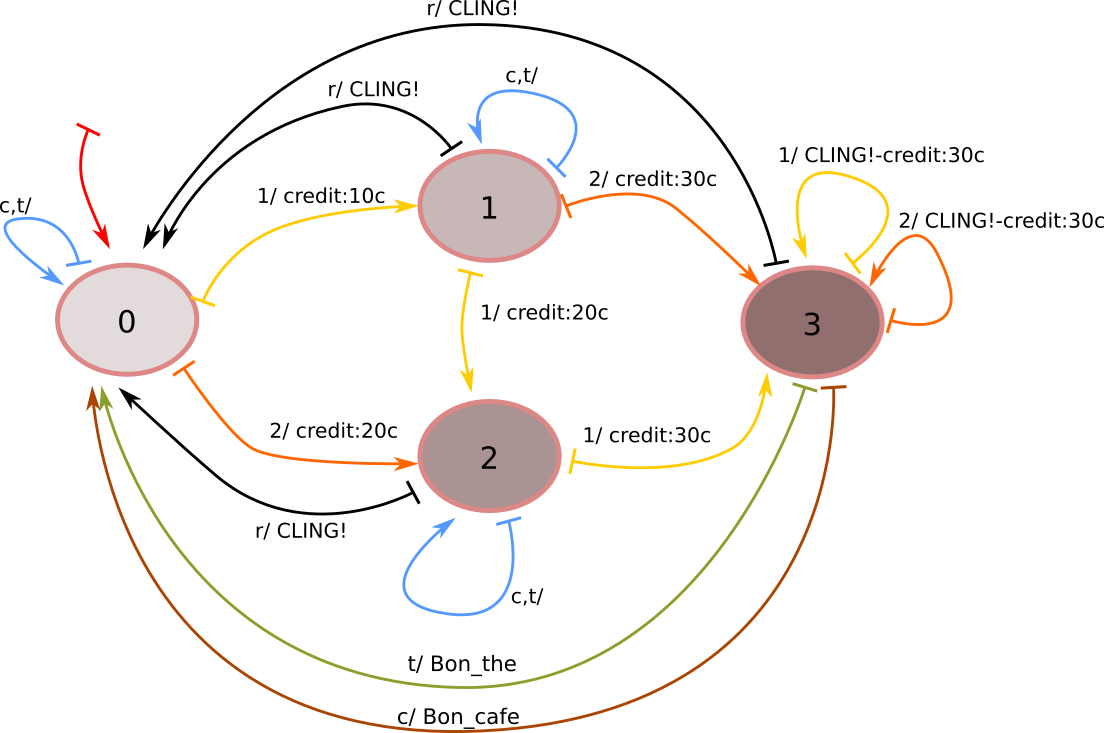
\includegraphics[width = 0.75\textwidth]{automate.png}
	\caption{Automate de machine à café. "\texttt{x/ sortie}" représente l'entrée \texttt{x} et la \texttt{sortie} correspondante, pouvant être nulle dans certains cas.}
\end{figure}
%\end{landscape}
%\newpage

[h]
\begin{lstlisting}[numbers=left, firstnumber = 0 ]
[~/INF203/TP9]: cat Cafe2/Automate_the.auto
4
0
18
0 c 0
0 t 0
0 1 1
0 2 2
1 c 1
1 t 1
1 r 0
1 1 2
1 2 3
2 c 2
2 t 2
2 r 0
2 1 3
3 1 3
3 2 3
3 r 0
3 c 0
3 t 0
12
0 1 credit:10c
0 2 credit:20c
1 1 credit:20c
1 2 credit:30c
1 r CLING!
2 r CLING!
2 1 credit:30c
3 r CLING!
3 1 CLING!-credit:30c
3 2 CLING!-credit:30c
3 c Bon_café
3 t Bon_thé

\end{lstlisting}

\begin{lstlisting}
[~/INF203/TP9]: ./caf2 Cafe2/Automate_the.auto
2
credit:20c
1
credit:30c
1
CLING!-credit:30c
t
Bon_thé
1
credit:10c
1
credit:20c
1
credit:30c
c
Bon_café
2
credit:20c
r
CLING!
q
\end{lstlisting}

%\newpage

\section{Un automate mystère}

[i]
L'état final est quand on arrive à écrire le mot BARBARA.

\begin{lstlisting}[numbers=left, firstnumber = 82 ]
[~/INF203/TP9]: tail -n 15 Mystere/automate.c
void simule_automate(automate * A) {
  int etat_courant, etat_suivant;
  int entree = ' ';

  etat_courant = A->etat_initial;
  while (entree != 'q' && A->etats_finals[etat_courant] != 1) {
    entree = lire_entree();
    if(entree!='q'){
      etat_suivant = A->transitions[etat_courant][entree];
      printf("%s\n", A->sortie[etat_courant][entree]);
      etat_courant = etat_suivant;
    }
  }
}
\end{lstlisting}



%\newpage
%\begin{landscape}
\begin{figure}[h]
	\centering
	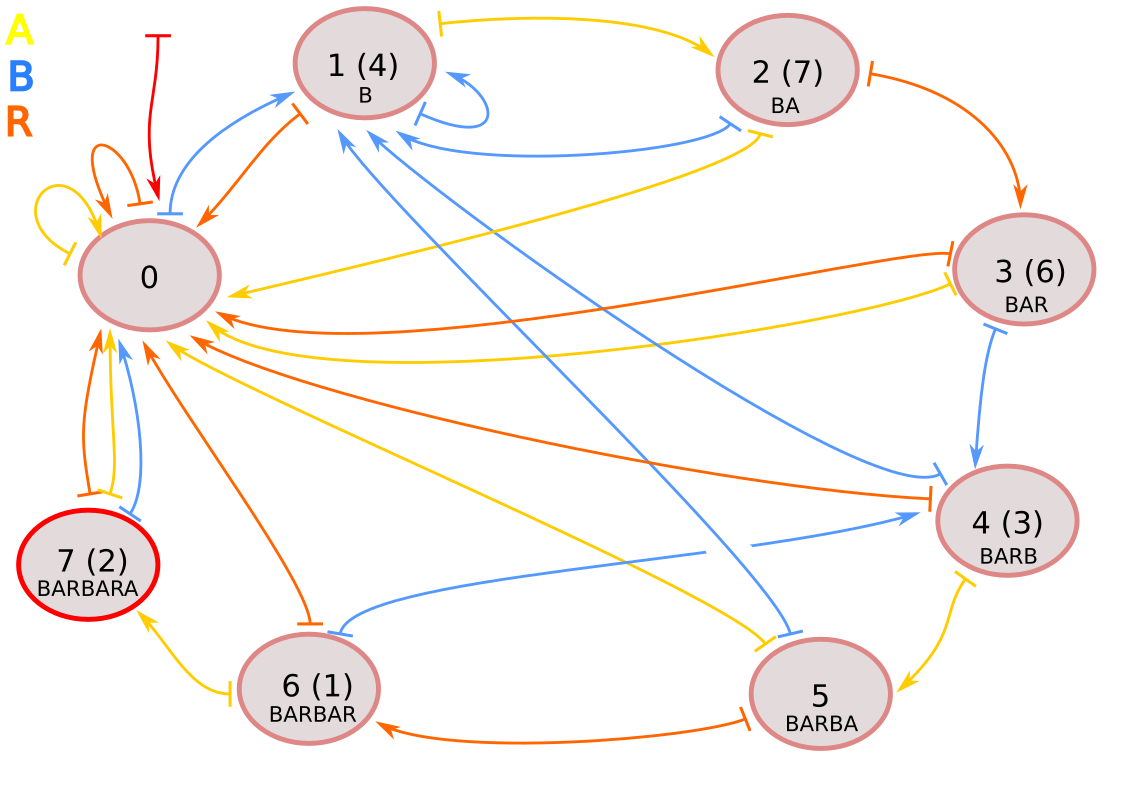
\includegraphics[width = 0.75\textwidth]{barbara.png}
	\caption{Automate de Barbara. La flèche rouge indique le départ et le rond rouge l'état final. Entre parenthèse figurent les états tels qu'inscrits dans le fichier de départ.}
\end{figure}
%\end{landscape}
%\newpage

\textit{L'automate était initialement dessiné avec les sorties sur BBB, mais la fermeture nous a surpris et nous avons tout perdu. Nous n'avons pas tout recopié pour ne pas surcharger la figure.}

%%%%%%%%%%%%%%%%%%%%%%%%%%%%%%%%%%%%%%%%%%%%%%%%%%%%%%%%%%%%%%%%%%%%%%
% Références
%%%%%%%%%%%%%%%%%%%%%%%%%%%%%%%%%%%%%%%%%%%%%%%%%%%%%%%%%%%%%%%%%%%%%%
%\newpage
\cite{}
%\subsection*{Bibliographie}
\bibliographystyle{authordate1}
\bibliography{ICU}

\end{document}